% Options for packages loaded elsewhere
\PassOptionsToPackage{unicode}{hyperref}
\PassOptionsToPackage{hyphens}{url}
\documentclass[12pt, ]{article}

\usepackage{mathtools}
\usepackage{amsmath}
\usepackage{amsthm}
\usepackage{amssymb}
\usepackage[italicdiff]{physics}
\mathtoolsset{showonlyrefs}

% SPACING AND FONTS %%%%%%%%%%%%%%%%%%%%%%%%%%%%%%%%%%%%%%%%%%%%%%%%%%%%%%%%%%%%
\usepackage{iftex}
% CAREFUL: the order of font includes here is very important!
\ifPDFTeX
  \usepackage[OT1,T1]{fontenc}
  \usepackage[utf8]{inputenc}
  \usepackage{textcomp} % provide euro and other symbols
    \usepackage[p,osf,swashQ]{cochineal}
  \usepackage[cochineal,vvarbb]{newtxmath}
      \usepackage[scale=0.95]{biolinum}
    \usepackage[scale=0.95,varl]{inconsolata}
\else % if luatex or xetex
  \usepackage[scale=0.95,varl]{inconsolata}
  \usepackage{newpxtext}
  \usepackage{mathpazo}
    \usepackage[scale=0.95]{biolinum}
  \fi
\ifLuaTeX
  \usepackage{selnolig}  % disable illegal ligatures
\fi
\IfFileExists{microtype.sty}{% use microtype if available
  \usepackage[]{microtype}
  \UseMicrotypeSet[protrusion]{basicmath} % disable protrusion for tt fonts
}{}

\setlength{\parindent}{0pt}
\setlength{\parskip}{10pt plus 2pt minus 2pt}
\setlength{\emergencystretch}{3em} % prevent overfull lines
\widowpenalty=10000
\clubpenalty=10000
\flushbottom
\allowdisplaybreaks
\sloppy


% CORE PACKAGES %%%%%%%%%%%%%%%%%%%%%%%%%%%%%%%%%%%%%%%%%%%%%%%%%%%%%%%%%%%%
\usepackage[dvipsnames,svgnames,x11names]{xcolor}
\usepackage[lmargin=1.5in,rmargin=1.5in,tmargin=1.2in,bmargin=1.2in]{geometry}
\usepackage[format=plain,
  labelfont={bf,sf,small,singlespacing},
  textfont={sf,small,singlespacing},
  justification=justified,
  margin=0.25in]{caption}

% SECTIONS AND HEADINGS %%%%%%%%%%%%%%%%%%%%%%%%%%%%%%%%%%%%%%%%%%%%%%%%%%%%%%%%
\setcounter{secnumdepth}{4}
\usepackage{sectsty}
\usepackage[compact]{titlesec}
% short title
\makeatletter
\newcommand\@shorttitle{}
\newcommand\shorttitle[1]{\renewcommand\@shorttitle{#1}}
\usepackage{fancyhdr}
\fancyhf{}
\pagestyle{fancy}
\renewcommand{\headrulewidth}{0pt}
\fancyheadoffset{0pt}
%\lhead{\scshape \@shorttitle}
%\rhead{\scshape\today}
\cfoot{\thepage}
\makeatother
% abstract styling
\renewenvironment{abstract}{
  \centerline
  {\large\sffamily\bfseries Abstract}\vspace{-1em}
  \begin{quote}\small
}{
  \end{quote}
}

% PANDOC INCLUDES %%%%%%%%%%%%%%%%%%%%%%%%%%%%%%%%%%%%%%%%%%%%%%%%%%%%%%%%%%%%%%

\providecommand{\tightlist}{%
  \setlength{\itemsep}{0pt}\setlength{\parskip}{0pt}}\usepackage{longtable,booktabs,array}
\usepackage{calc} % for calculating minipage widths
% Correct order of tables after \paragraph or \subparagraph
\usepackage{etoolbox}
\makeatletter
\patchcmd\longtable{\par}{\if@noskipsec\mbox{}\fi\par}{}{}
\makeatother
% Allow footnotes in longtable head/foot
\IfFileExists{footnotehyper.sty}{\usepackage{footnotehyper}}{\usepackage{footnote}}
\makesavenoteenv{longtable}
\usepackage{graphicx}
\makeatletter
\def\maxwidth{\ifdim\Gin@nat@width>\linewidth\linewidth\else\Gin@nat@width\fi}
\def\maxheight{\ifdim\Gin@nat@height>\textheight\textheight\else\Gin@nat@height\fi}
\makeatother
% Scale images if necessary, so that they will not overflow the page
% margins by default, and it is still possible to overwrite the defaults
% using explicit options in \includegraphics[width, height, ...]{}
\setkeys{Gin}{width=\maxwidth,height=\maxheight,keepaspectratio}
% Set default figure placement to htbp
\makeatletter
\def\fps@figure{htbp}
\makeatother
% END PANDOC %%%%%%%%%%%%%%%%%%%%%%%%%%%%%%%%%%%%%%%%%%%%%%%%%%%%%%%%%%%%%%%%%%%

% USER INCLUDES %%%%%%%%%%%%%%%%%%%%%%%%%%%%%%%%%%%%%%%%%%%%%%%%%%%%%%%%%%%%%%%%
% additional LaTeX code for the "preamble" goes here
\makeatletter
\makeatother
\makeatletter
\makeatother
\makeatletter
\@ifpackageloaded{caption}{}{\usepackage{caption}}
\AtBeginDocument{%
\ifdefined\contentsname
  \renewcommand*\contentsname{Table of contents}
\else
  \newcommand\contentsname{Table of contents}
\fi
\ifdefined\listfigurename
  \renewcommand*\listfigurename{List of Figures}
\else
  \newcommand\listfigurename{List of Figures}
\fi
\ifdefined\listtablename
  \renewcommand*\listtablename{List of Tables}
\else
  \newcommand\listtablename{List of Tables}
\fi
\ifdefined\figurename
  \renewcommand*\figurename{Figure}
\else
  \newcommand\figurename{Figure}
\fi
\ifdefined\tablename
  \renewcommand*\tablename{Table}
\else
  \newcommand\tablename{Table}
\fi
}
\@ifpackageloaded{float}{}{\usepackage{float}}
\floatstyle{ruled}
\@ifundefined{c@chapter}{\newfloat{codelisting}{h}{lop}}{\newfloat{codelisting}{h}{lop}[chapter]}
\floatname{codelisting}{Listing}
\newcommand*\listoflistings{\listof{codelisting}{List of Listings}}
\makeatother
\makeatletter
\@ifpackageloaded{caption}{}{\usepackage{caption}}
\@ifpackageloaded{subcaption}{}{\usepackage{subcaption}}
\makeatother
\makeatletter
\@ifpackageloaded{tcolorbox}{}{\usepackage[skins,breakable]{tcolorbox}}
\makeatother
\makeatletter
\@ifundefined{shadecolor}{\definecolor{shadecolor}{rgb}{.97, .97, .97}}
\makeatother
\makeatletter
\makeatother
\makeatletter
\makeatother
% END USER INCLUDES %%%%%%%%%%%%%%%%%%%%%%%%%%%%%%%%%%%%%%%%%%%%%%%%%%%%%%%%%%%%

% BIBLIOGRAPHY %%%%%%%%%%%%%%%%%%%%%%%%%%%%%%%%%%%%%%%%%%%%%%%%%%%%%%%%%%%%%%%%%
\usepackage[]{natbib}
\bibliographystyle{apalike}

% Give it this name so that it works with ::: #refs
\newenvironment{CSLReferences}[2]{
\bibliography{bibliography.bib}
\clearpage
}{}

% LINKS %%%%%%%%%%%%%%%%%%%%%%%%%%%%%%%%%%%%%%%%%%%%%%%%%%%%%%%%%%%%%%%%%%%%%%%%
\usepackage{hyperref}
\usepackage{url}
\hypersetup{
  pdftitle={The 2/3 Accuracy Ceiling \& Why We Should Rethink Letting AI Predict Recidivism: A Replication of Dressel \& Farid (2018)},
  pdfauthor={Mark Ayiah \& Gabi Picott},
  colorlinks=true,
  linkcolor={black},
  filecolor={Maroon},
  citecolor={VioletRed4},
  urlcolor={DodgerBlue4},
  pdfcreator={LaTeX via pandoc}}

% TITLE, AUTHOR, DATE %%%%%%%%%%%%%%%%%%%%%%%%%%%%%%%%%%%%%%%%%%%%%%%%%%%%%%%%%%
\title{\sffamily\bfseries\huge\parfillskip=0pt
\rightskip=0pt plus .5\textwidth
\leftskip=0pt plus .5\textwidth
\emergencystretch=.3\textwidth The 2/3 Accuracy Ceiling \& Why We Should
Rethink Letting AI Predict Recidivism: A Replication of Dressel \& Farid
(2018)}
\shorttitle{The 2/3 Accuracy Ceiling \& Why We Should Rethink Letting AI Predict Recidivism: A Replication of Dressel \& Farid (2018)}
\author{\textbf{Mark Ayiah \& Gabi Picott}
 }
\date{}


\begin{document}
\allsectionsfont{\sffamily}

\maketitle

\begin{abstract}
In the modern criminal justice system, machine learning algorithms are
commonly used to predict a defendant's likelihood of recidivating, or
repeating an offense. The risk assessment software COMPAS is one of the
most widely used tools to do this, but research by Dressel \& Farid
finds that COMPAS' predictions plateau at an accuracy rate of
approximately 67\%, a rate identical to that of the judgment of people
with no special knowledge of the criminal justice system and of models
much less complex than COMPAS. We formulate two logistic regression
models with the features specified by Dressel \& Farid and also find
that these models are accurate only two-thirds of the time. We then
build upon their results by calculating precision, recall, and F-1 Score
to delve deeper into the reliability, or lack thereof, of employing
machine learning algorithms for predicting recidivism. Our analysis
supports Dressel \& Farid's notion that these algorithms have limited
predictive power and may be too haphazard to be relied on in the
criminal justice field.
\end{abstract}

\ifdefined\Shaded\renewenvironment{Shaded}{\begin{tcolorbox}[enhanced, sharp corners, interior hidden, boxrule=0pt, frame hidden, borderline west={3pt}{0pt}{shadecolor}, breakable]}{\end{tcolorbox}}\fi



% USER BODY %%%%%%%%%%%%%%%%%%%%%%%%%%%%%%%%%%%%%%%%%%%%%%%%%%%%%%%%%%%%%%%%%%%%

\emph{Link to GitHub repository:
\url{https://github.com/mark-ayiah/aqrd23-final-project/tree/main}}

\hypertarget{introduction-and-theory}{%
\section{Introduction and Theory}\label{introduction-and-theory}}

In an age where artificial intelligence (AI) and machine learning are
becoming more advanced and ubiquitous, many fields are trying to
incorporate these methods into their practices to improve the efficiency
of their work. The Criminal Justice and Legal System is no exception to
this, as for the past two decades, machine learning algorithms and AI
have been used by judges, parole officers and other key figures within
the courts and prison systems for predictive purposes. These algorithms
have been used to anticipate whether defendants will miss court
hearings, who is most likely to commit a violent crime, and where crimes
will most likely occur (Perry et al., 2013).\footnote{Perry, W. L.,
  McInnis, B., Price, C. C., Smith, S. C., \& Hollywood, J. S. (2013).
  Predictive Policing: The Role of Crime Forecasting in Law Enforcement
  Operations. RAND Corporation.
  \url{http://www.jstor.org/stable/10.7249/j.ctt4cgdcz}} One of the most
pertinent uses of these machine learning techniques is predicting
recidivism, or whether an offender will offend again.

Correctional Offender Management Profiling for Alternative Sanctions, or
COMPAS, is a widely used software that predicts whether an offender will
commit a misdemeanor or felony within 2 years of being evaluated. COMPAS
is designed to make these predictions using a total of 137 distinct
features about each offender and their past criminal record. Although
the long list of features COMPAS uses does not explicitly include race,
scholars have claimed that the algorithm is biased against Black
defendants. In 2016, Angwin analyzed COMPAS by comparing the risk scores
it assigned to the same Broward County defendant dataset used in
\citep{dressel2018accuracy}. They found that Black defendants are nearly
twice as likely as White descendants to be misclassified as high risk.
Regardless of race, only 61\% of those predicted to recidivate actually
did so, and the algorithm was overall only a little more accurate than a
``coin flip'' (Angwin et al., 2016).\footnote{Angwin, J., Larson, J.,
  Kirchner, L., \& Mattu, S. (2016, May 23). Machine bias. ProPublica.
  \url{http://www.propublica.org/article/machine-bias-risk-assessments-in-criminal-sentencing}}
Whether or not racial disparities can be attributed to bias is still
debated amongst researchers, but the model appears to perform
haphazardly regardless of the defendant's race.

Though it is prevalent in research, COMPAS is certainly not the only
machine learning tool or algorithm that has been developed to predict
recidivism. A recent study that analyzed the Broward County data using
K-Nearest Neighbors, Random Forest, Support Vector Machine, and Logistic
Regression found the predictive accuracy rates of all the models to fall
between 64\% to 67\% and have AUC values between 0.65 to 0.72 (Zhang,
2022).\footnote{Zhang, J. (2023). Research on the criminal recidivism
  prediction based on machine learning algorithm. Proceedings of the
  2022 2nd International Conference on Business Administration and Data
  Science (BADS 2022), 1297--1306.
  \url{https://doi.org/10.2991/978-94-6463-102-9_134}} Their findings
are extremely similar to those of Dressel \& Farid, whose two logistic
regression models and SVM model all have accuracy rates between 64.3\%
and 66.8\%. It appears that scholars often reach an accuracy plateau
when analyzing the accuracy of their algorithms for predicting
recidivism. In this paper, we replicate and analyze the logistic
regression models of Dressel \& Farid, and also calculate precision and
accuracy metrics to try to understand the effectiveness of these models.

In this paper, we begin our analysis by calculating accuracy rates,
false negatives, and false positives using the COMPAS predictions from
the Broward County data. We then construct and train a 7-feature and
2-feature logistic classification model utilizing the same unique
predicting features as Dressel \& Farid in their respective models. In
addition to replicating Dressel \& Farid's methodology, we calculate
confusion matrices during the training of our logistic regression
models. From these matrices, we derive precision and recall metrics,
which reveal that our models can accurately identify slightly over half
of the defendants who recidivate. However, they also tend to falsely
classify about half of these individuals as not at risk of recidivism.
Knowing our classifier produces accuracies in close proximity to
COMPAS', these results raise serious questions about the reliability of
machine learning algorithms in making these critical decisions.

\hypertarget{data-and-methods}{%
\section{Data and Methods}\label{data-and-methods}}

\hypertarget{tbl-1}{}
\begin{longtable}[]{@{}l@{}}
\caption{\label{tbl-1}Defendant Summary Statistics}\tabularnewline
\toprule\noalign{}
\endfirsthead
\endhead
\bottomrule\noalign{}
\endlastfoot
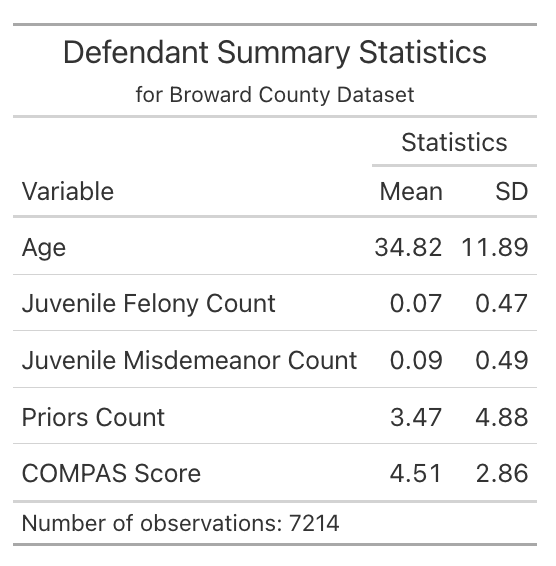
\includegraphics{tables/tbl1.png} \\
\end{longtable}

We utilized the Broward County dataset, as employed by Dressel \& Farid
(2018), to construct, train, and analyze our logistic classification
models. This dataset consists of comprehensive information on 7,214
pre-trial defendants from Broward County, FL, including demographic
details, criminal history, COMPAS recidivism risk scores, and arrest
records 2 years following COMPAS assessment. The COMPAS decile scores
range from 1 to 10. Recidivism risk is classified as low (1 to 4),
medium (5 to 7), and high (8 to 10). A positive COMPAS prediction,
signifying a defendant will recidivate, corresponds to decile scores
above 4, while a negative prediction corresponds to scores equal to or
less than 4. See Table 1 for a summary of key characteristics of
defendants in the dataset. See Table 7 and 8 in the appendix for summary
statistics for Black (Table 7) and White (Table 8) defendants
separately.

We employed two primary models devised by Dressel \& Farid (2018) for
our replication and extension of their recidivism prediction results.
Both models utilize a logistic regression framework expressed as:

\[ \Pr(\boldsymbol{Y}_i = 1) =   \dfrac{\exp(\boldsymbol{X}_i^T\boldsymbol{\beta})}{1+\exp(\boldsymbol{X}_i^T\boldsymbol{\beta})} \]

Where \(Y_i\) is a binary response variable that indicates whether or
not defendant \(i\) recidivates. \(Y_i = 0\) denotes the case where
defendant \(i\) does not recidivate, and \(Y_i = 1\) denotes the case
where defendant \(i\) does recidivate. For the 7-feature model,
\(\boldsymbol{X}_i^T\) denotes the \(1 \times 7\) covariate matrix for
observation \(i\), representing the 7 covariates of age, sex, number of
juvenile misdemeanor charges, number juvenile felony charges, number of
prior non-juvenile charges, specific crime charge, and crime degree, and
\(\boldsymbol{\beta}\) denotes the \(7 \times 1\) vector of estimated
regression coefficients for those same 7 features.

The second model that we use only incorporates 2 features, but utilizes
the same logistic regression framework as above. The only differences in
the two models are that \(\boldsymbol{X}_i^T\) denotes the
\(1 \times 2\) covariate matrix for observation \(i\), representing the
2 covariates of age and number of prior non-juvenile charges, and
\(\boldsymbol{\beta}\) denotes the \(2 \times 1\) vector of estimated
regression coefficients for those same 2 features.

As outlined in Dressel \& Farid (2018), we trained both models on 1000
different 80\%/20\% training/test splits from the full Broward County
dataset. After bootstrapping, we calculated 95\% confidence intervals
for the average estimates of the models' overall accuracy rate, accuracy
rate for White and Black defendants, false positive rates for White and
Black defendants, and false negative rates for White and Black
defendants. We also aggregated the predictions from all 1000 iterations
of training the models to create confusion matrices, from which we
calculated the following performance metrics: accuracy, precision,
recall, F1 score, false negative rate, and false positive rate for all
defendants included in the Broward County dataset. Table 5 and 6 (see
appendix) summarize the classification results of our 7-feature Model
and 2-feature Models, respectively, after training 1000 times with a
80\%/20\% training/testing split on the Broward County Data in a
confusion matrix. The metrics in Table 4 were calculated with the
following formulas from all data points over the 1000 training
iterations:

\(\text{Accuracy} = \frac{\text{True Positives} + \text{True Negatives}}{\text{Total Instances}}\\\\ \text{Precision} = \frac{\text{True Positives}}{\text{True Positives} + \text{False Positives}}\\\\ \text{Recall} = \frac{\text{True Positives}}{\text{True Positives} + \text{False Negatives}}\\\\ \text{F1 Score} = 2 \times \frac{\text{Precision} \times \text{Recall}}{\text{Precision} + \text{Recall}}\\\\ \text{False Negative Rate} = \frac{\text{False Negatives}}{\text{False Negatives} + \text{True Positives}}\\\\ \text{False Positive Rate} = \frac{\text{False Positives}}{\text{False Positives} + \text{True Negatives}}\)

The basic assumptions required for logistic regression include the
independence of observations, the binary nature of the response
variable, the lack of outliers or strongly influential points, minimal
multicollinearity between the covariates, and a linear relationship
between the explanatory variables and the log odds of the response
variable. All of these assumptions hold for our dataset.

\hypertarget{results}{%
\section{Results}\label{results}}

\hypertarget{tbl-2}{}
\begin{longtable}[]{@{}l@{}}
\caption{\label{tbl-2}COMPAS Algorithmic Predictions}\tabularnewline
\toprule\noalign{}
\endfirsthead
\endhead
\bottomrule\noalign{}
\endlastfoot
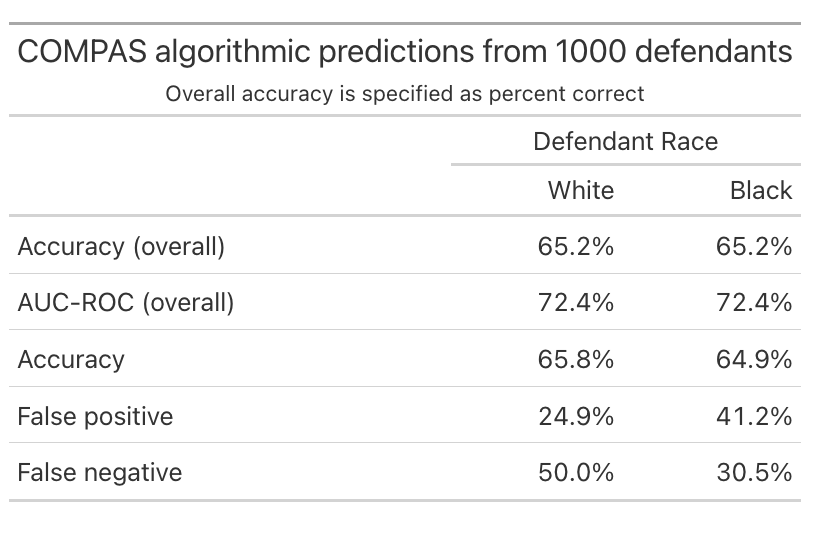
\includegraphics{tables/tbl2.png} \\
\end{longtable}

Table 2 replicates Table 1 in Dressel \& Farid (2018), summarizing
COMPAS predictions for Black and White defendants from a subset of 1,000
defendants in the Broward County dataset. The accuracy for the entire
subset was 65.2\%, with an overall AUC-ROC of 0.724. Notable disparities
emerged when defendants were separated by race. While accuracy rates
were relatively close---64.9\% for Black defendants and 65.8\% for White
defendants---significant differences were observed in false positive and
false negative rates. The false positive rate for Black defendants was
65.5\% higher than the false positive rate for White defendants. Black
defendants had a false positive rate of 41.2 percent compared to the
White defendants' false positive rate of 24.9 percent. Conversely, the
false negative rate for Black defendants was 39\% lower than the false
negative rate for White defendants. Black defendants had a false
negative rate of 30.5 \% compared to the White false negative rate of
50.0\%. Dressel \& Farid (2018) conducted an unpaired t-test, revealing
significant differences in the false positive and negative rates across
race (p = 0.001 and p = 0.030, respectively). We only had access to the
one subset of defendants used in the Human Assessment part of Dressel \&
Farid's study, whereas they had several, so we could not perform an
unpaired t-test. However, the similarity of accuracy rates across race
and noteable distance between false positive and negatives rates suggest
a statistically significant difference.

\hypertarget{tbl-3}{}
\begin{longtable}[]{@{}l@{}}
\caption{\label{tbl-3}Logistic Regression Algorithmic
Predictions}\tabularnewline
\toprule\noalign{}
\endfirsthead
\endhead
\bottomrule\noalign{}
\endlastfoot
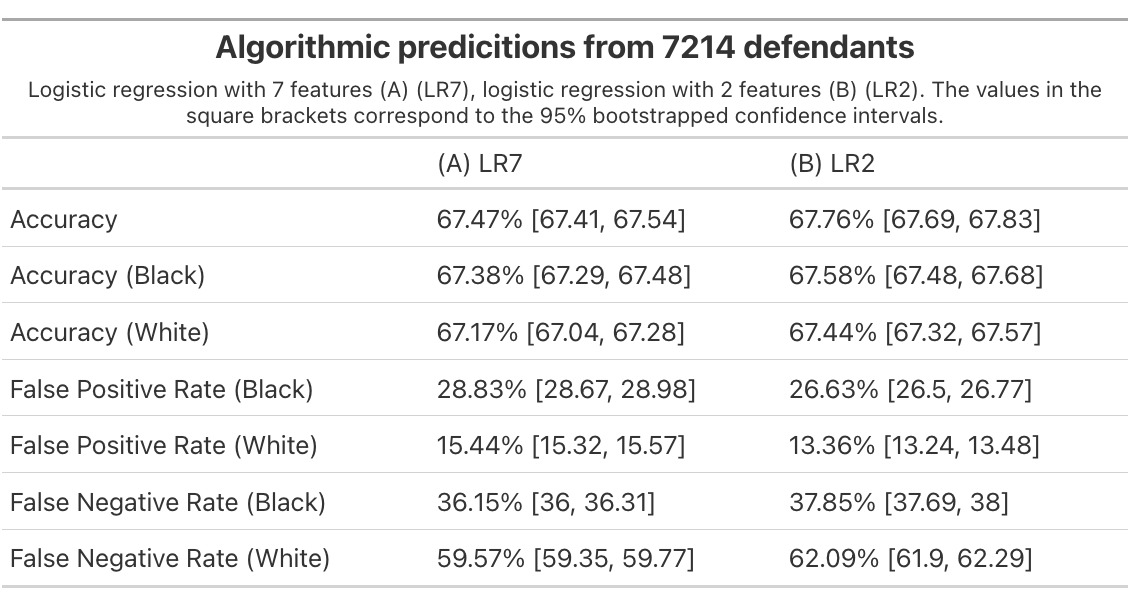
\includegraphics{tables/tbl3.png} \\
\end{longtable}

Table 3 replicates columns (A) and (B) of Table 2 from Dressel \& Farid
(2018) and displays measures of the accuracy and fairness across racial
lines for the 7-feature and 2-feature logistic regression models. The
overall accuracies between models are highly comparable, with values of
67.5\% and 67.8\%respectively. The accuracy stays at the two-thirds
ceiling for both Black and White defendants in both models as well.
However, sizable differences are seen in the false positive and false
negative rates between Black and White defendants for both models, with
White defendants having much higher false negative rates and much lower
false positive rates than Black defendants. This echoes the biases found
in the COMPAS predictions, indicating similar levels and directions of
unfairness as the COMPAS model and the participants of the Dressel \&
Farid (2018) study.

\hypertarget{tbl-4}{}
\begin{longtable}[]{@{}l@{}}
\caption{\label{tbl-4}Performance Metrics}\tabularnewline
\toprule\noalign{}
\endfirsthead
\endhead
\bottomrule\noalign{}
\endlastfoot
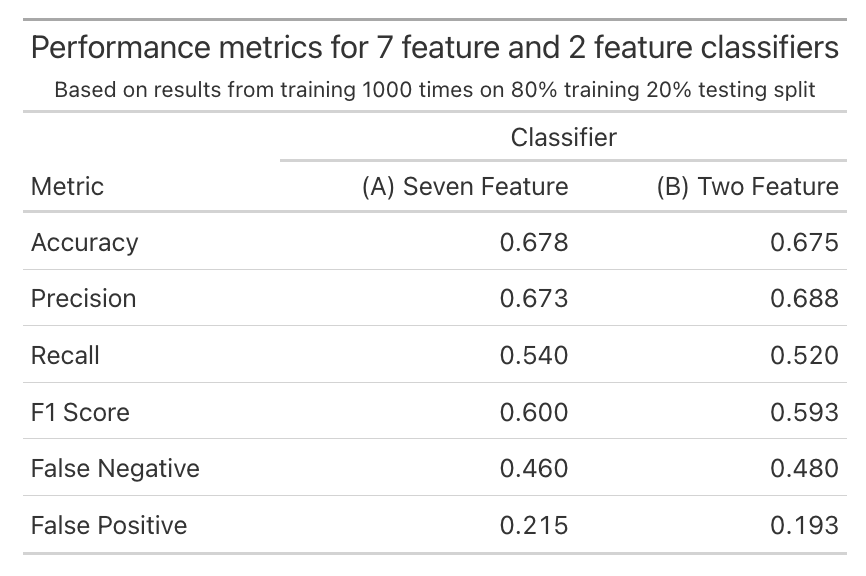
\includegraphics{tables/tbl4.png} \\
\end{longtable}

Table 4 summarizes the precision, recall, and accuracy metrics
calculated from the results in Table 5 and Table 6 (see appendix). These
tables present the confusion matrices of our 7-feature and 2-feature
classifying models. Both classifiers had very similar average accuracy
rates, with the 7-feature model correctly classifying defendants 67.8\%
of the time and the 2-feature model correctly classifying defendants
67.5\% of the time. These percentages represent the proportion of our
models' correct predictions out of all predictions they made, indicating
that both models made predictions that were correct around two-thirds of
the time. The 7-feature model and the 2-feature model showcase false
negative rates of 46\% and 48\%, respectively. This implies that the
more complex model was marginally more accurate, although both models
falsely classified defendants as not at risk of recidivating nearly half
of the time. The false positive rates were relatively low, with a rate
of 21.5\% for the 7-feature model and 19.3\% for the 2-feature model.
This time, the simpler model was marginally more accurate, yet both
models falsely classify defendants as at risk of recidivating
approximately one fifth of the time. These accuracy rates echo the
overall accuracy rates that COMPAS, the two logistic regression models,
and the SVM model achieved in Dressel \& Farid (2018), though the ones
we calculated are marginally higher. It should be noted, again, that the
majority of the accuracy rates appear to reach a maximum of only 1 or 2
percentage points over 67\%, if they even do approach that level of
predictive accuracy.

The 7-feature model and 2-feature model displayed precision rates of
67.3\% and 68.8\%, respectively. This signifies that, of the defendants
predicted to likely recidivate by the 7-feature model, 67.3\% actually
did, while the 2-feature model had a slightly higher precision of 68.8\%
in predicting this. These precision rates suggest the 2-feature model
has a marginal advantage in identifying defendants at a high risk of
recidivating. Nevertheless, both models consistently demonstrate the
ability to reliably identify high-risk defendants around two-thirds of
the time.

In contrast to the accuracy and precision rates, the recall rates for
both the 7-feature and 2-feature models were relatively lower. The
recall rate provides an idea of the sensitivity of the models, or in
other words, the probability that an actual positive will be classified
as positive.

The 7-feature model exhibited a recall rate of 54\%, while the 2-feature
model performed slightly worse with a rate of of 52\%. These rates
indicate that the models successfully identified 54\% and 52\% of
individuals who eventually recidivated, respectively. In context, these
results suggest that both models are able to correctly classify a little
over half of the defendants who recidivate as at-risk, but classify the
other half as not at-risk.

The F1 scores of both models, 0.6 for the 7-feature model and 0.593 for
the 2-feature model, utilize the harmonic mean of precision and recall,
creating a more balanced metric to describe their accuracy in predicting
recidivism. Their similar F1 scores indicate that both models strike a
reasonable balance between precision and recall, and perform better than
average at correctly identifying individuals at risk of recidivating
while simultaneously capturing a substantial proportion of those who do
recidivate.

\hypertarget{discussion-and-conclusion}{%
\section{Discussion and Conclusion}\label{discussion-and-conclusion}}

The results of our replication and extension of the Dressel \& Farid
(2018) study further confirm the limited predictive ability of machine
learning models for recidivism prediction. We found that across all of
the models, ranging from very complex (137-feature COMPAS model) to very
simple (2-feature logistic regression), predictive accuracy for
recidivism consistently reaches a ceiling of approximately 67\%
correctness. While it remains to be seen if there are more informative
features about defendants that have yet to be discovered or tested, our
replication of Dressel \& Farid's analysis signals that a predictive
accuracy of two-thirds may be the practical limit for the available data
and tools.

Further, our replication and extension further draw out and confirm
concerning racial disparities in the error rates of predictive models
between Black and White defendants. Though overall predictive accuracy
is comparable between groups, Black defendants are more likely to be
incorrectly classified as high risk, while more White defendants are
overlooked as low risk. This indicates that machine learning models may
disproportionately target Black defendants, and with how widely used
tools like COMPAS are and will continue to become, this unveils a
concerning reality for the future of the justice system as it relates to
racial inequity. Thus, policymakers should explore alternative
approaches to promoting public safety and rehabilitation that do not
perpetuate racial inequities and discriminatory practices. More research
is necessary to develop improved predictive models or identify better
solutions altogether.

Lastly, the results of our extension provide deeper insight into the
accuracy and implications of using machine learning algorithms to
predict recidivism. As expected, the 7-feature and 2-feature logistic
regression models demonstrated accuracy rates that indicate a predictive
power of approximately two-thirds for both models, which is a little
higher than that of COMPAS (65.2\% overall). Similarly, the precision of
both models indicate that approximately two-thirds of the individuals
that the models predict will recidivate actually go on to recidivate.
While this appears to suggest a high or at least expected predictive
power for the models, the comparatively low recall rates should be
noted. The models' recall rates suggest that the models correctly
capture those who recidivate approximately half of the time, but
simultaneously falsely classify recidivists as not at-risk about half
the time. Our findings align with those of researchers such as Angwin et
al.~(2016), who claimed that the algorithm they used to classify
individuals in the Broward County dataset exhibited an accuracy slightly
higher than chance, similar to a coin flip with a 50\% likelihood in
either direction.

Machine learning models like ours exhibit a precision-recall trade off,
and researchers often aim to strike a balance by maximizing the F1
score. Researchers who want to improve algorithms that predict
recidivism must consider what type of accuracy is most important. If
researchers care more about minimizing missed cases, they should
prioritize creating models with higher recall, even at the cost of lower
precision. Conversely, if they want to minimize false positives, they
should prioritize creating models with higher precision, which will lead
to lower recall. In any case, these findings raise concerns about the
real-world performance of machine learning algorithms in recidivism
prediction, and should urge researchers to more closely and carefully
examine how they are being developed and deployed.

\hypertarget{refs}{}

\begin{CSLReferences}{0}{0}\end{CSLReferences}

\appendix

\hypertarget{appendix}{%
\section{Appendix}\label{appendix}}

\hypertarget{tbl-5}{}
\begin{longtable}[]{@{}l@{}}
\caption{\label{tbl-5}7-Feature Model Confusion Matrix}\tabularnewline
\toprule\noalign{}
\endfirsthead
\endhead
\bottomrule\noalign{}
\endlastfoot
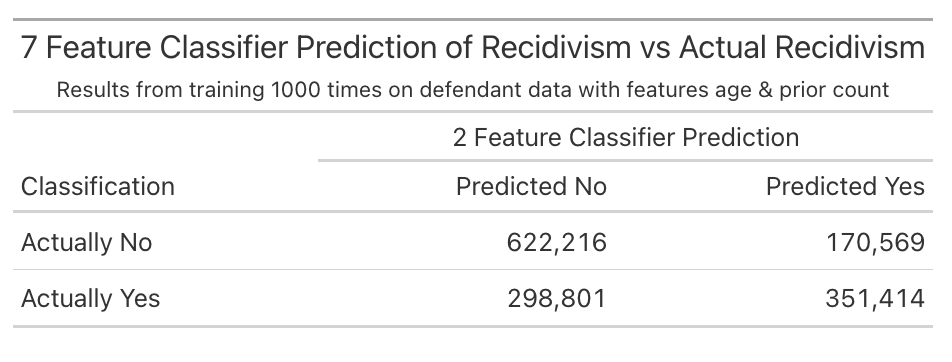
\includegraphics{tables/tbl5.png} \\
\end{longtable}

\hypertarget{tbl-6}{}
\begin{longtable}[]{@{}l@{}}
\caption{\label{tbl-6}2-Feature Model Confusion Matrix}\tabularnewline
\toprule\noalign{}
\endfirsthead
\endhead
\bottomrule\noalign{}
\endlastfoot
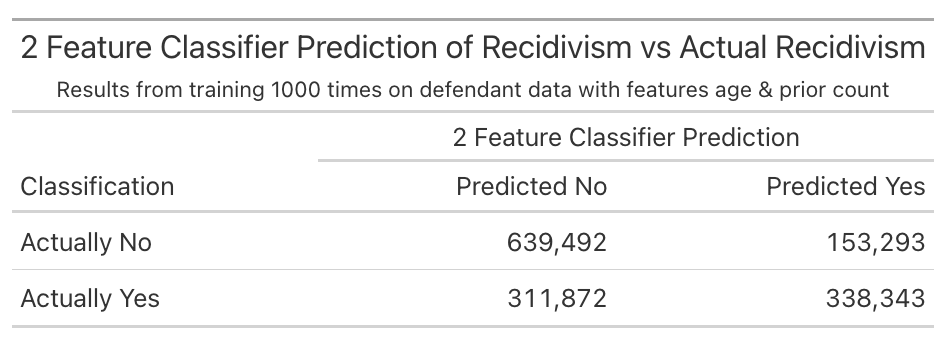
\includegraphics{tables/tbl6.png} \\
\end{longtable}

\hypertarget{tbl-7}{}
\begin{longtable}[]{@{}l@{}}
\caption{\label{tbl-7}Black Defendant Summary Statistics}\tabularnewline
\toprule\noalign{}
\endfirsthead
\endhead
\bottomrule\noalign{}
\endlastfoot
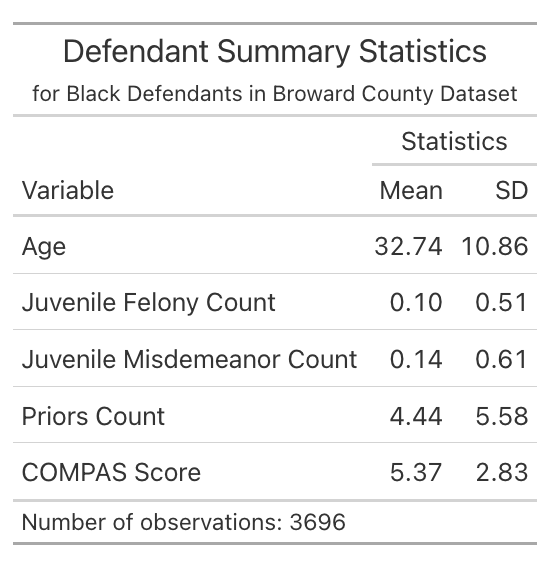
\includegraphics{tables/tbl7.png} \\
\end{longtable}

\hypertarget{tbl-8}{}
\begin{longtable}[]{@{}l@{}}
\caption{\label{tbl-8}White Defendant Summary Statistics}\tabularnewline
\toprule\noalign{}
\endfirsthead
\endhead
\bottomrule\noalign{}
\endlastfoot
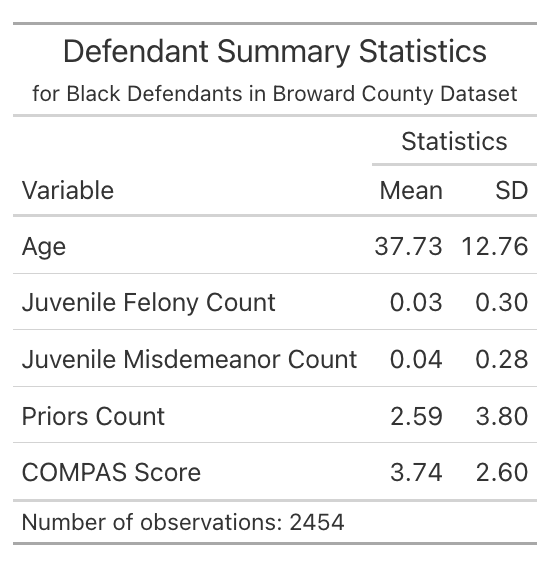
\includegraphics{tables/tbl8.png} \\
\end{longtable}

% END BODY %%%%%%%%%%%%%%%%%%%%%%%%%%%%%%%%%%%%%%%%%%%%%%%%%%%%%%%%%%%%%%%%%%%%%



\end{document}
